\documentclass[]{article}
\usepackage{listings}
\usepackage{hyperref}
\usepackage{xcolor}
\usepackage{geometry}
\usepackage{csquotes}
\usepackage[]{setspace}
\usepackage[]{graphicx}
\usepackage[]{amsmath}
\usepackage[]{amsfonts}
\usepackage[]{hyperref}
\usepackage{caption}
\usepackage{subcaption}
\usepackage{graphicx}
\usepackage[
backend=biber,
style=authoryear-comp,
sorting=ynt]{biblatex}
\addbibresource{phdreflib.bib}

\geometry{margin=1in}
\setlength{\parskip}{6pt}
\setlength\parindent{0pt}
\setstretch{1}

%opening
\title{From Neural to Social Computation: Collective Intelligence in Networks of Complex Agents}
\author{Marie-Lou Laprise\footnote{Some of the ideas for this project were developed in collaboration with Kamesh Krishnamurthy (Princeton Physics \& PNI)}}

\begin{document}
	
	\maketitle
\section{Introduction}

\rightline{``\textit{Think how hard physics would be if particles could think}" --Murray Gell-Mann}

A variety of complex systems across scales, from colonies of ants to neurons in the brain, map noisy inputs to useful outputs in a decentralized, emergent manner: they perform distributed computation.\footnote{ I loosely follow Crutchfield (\cite{crutchfieldCalculiEmergenceComputation1994}) by defining \textbf{computation} as a useful mapping from an input to an output; and \textbf{distributed} to mean that computation emerges from the time-varying state of a system of many interacting elements.} Repeated interactions in social networks also produce emergent computation; a prominent example being price discovery in financial markets. This remains a blind spot for both social science and theories of collective computation. 

\textbf{Nonlinearity.} In studies of opinion formation in control systems or social science, traditional opinion models relied on linear dynamics that have limited expressivity and cannot replicate threshold effects or information saturation. Meanwhile, in neuroscience or biophysics, rich and expressive nonlinear models of distributed computation have been developed and studied extensively.

\textbf{Heterogeneity.} Both nonlinear models from neuroscience and opinion formation models generally feature simple, homogeneous, and memory-less units (neurons or agents)--in the first case, for realism; in the second case, for tractability only. Social agents, however, are complex and heterogeneous. 

\textbf{General questions.} Can we extend nonlinear models of neural computation to explore how heterogeneous social agents collect and exchange noisy information to collectively form opinions and make decisions? How much heterogeneity and complexity can we add while keeping a tractable model that can be informative about social dynamics?

\textbf{Specific question.} As a first step, in this project, I examine how adaptive time constants change how networks of interacting agents break indecision in response to contradictory signals and form collective, stable opinion patterns.

\textbf{RNN model of opinion formation.} In recent work, Naomi Leonard and colleagues developed a model of multi-agent opinion formation that takes a form similar to a recurrent neural network (RNN) (\cite{bizyaevaNonlinearOpinionDynamics2022}, \cite{leonardFastFlexibleMultiAgent2024}) (the “BFL” model; see Section 2.1). They introduced nonlinearity to model information saturation, in contrast to linear averaging models that dominated the field of opinion dynamics. The BFL model is able to break indecision in the face of contradictory inputs. It rapidly converges to a steady state of consensus (all agents agree) or disagreement (agreement within subgroups but not between them) in a way that, its authors argue, parallels the observed behavior of bees choosing a nesting site or voters choosing a candidate.

\textbf{Contribution.} The BFL model features simple, homogeneous agents, without memory or intelligence. I take a first step towards richer agent-level behavior by adding an adaptive time constant (or gate) to the opinion update. I then examine the dynamics of the gated model for different signal strengths and different types of connectivity matrices, compared to the initial model, using simulations in Julia.

\section{Methods}
\subsection{The BFL model}

While the BFL model can model multi-opinion formation, here I focus on the case of two mutually exclusive opinions represented by a scalar value $z$. The agent favors a given option when $z>0$, he disfavors it when $z<0$, and he is neutral when $z = 0$.

Each agent is represented by coupled ODEs. Agents communicate through a connectivity network. The instantaneous rate of change of (1) the opinion $z$ of agent $i$ and (2) the susceptibility or excitability $u$ of agent $i$,\footnote{In the initial model, the $u$ term is called attention. Here, we call it susceptibility to avoid any confusion with other uses of the word attention in machine learning and neuroscience.} for a network of size $N$, are as follows:
\begin{align}
	\dot{z}_{i}(t) &= -d_{i}z_{i}(t) + S \left( u_i(t) \cdot  \sum^{N}_{j=1} J^z_{ij}z_{j}(t)  \right) + I_{i}(t) \\
	\tau^u \dot{u}_i(t) &= -u_i(t)+u_0+g^u \sum ^{N}_{j=1} J^u_{ij}(z_{j}(t))^2
\end{align}

\textbf{Differences with vanilla RNNs.} It should be emphasized at the outset that contrary to the traditional RNN case, each agent $i$ has access only to its own input $I_i$. The only way for an agent to access inputs that were distributed to other agents is indirectly, by communication through the adjacency graph. Contrary to RNNs in machine learning, parameters are not learned through back-propagation; they must be set as hyper-parameters (or could be learned locally). 

\textbf{Components of the opinion update.} In the opinion update, the first term corresponds to linear negative feedback or self-inhibition, the second term to nonlinear positive feedback or recurrent excitation, and the last term is a time-varying input $I_i(t)$ that includes external input (signal and noise) and internal bias.

\textbf{Role of susceptibility.} The susceptibility $u_i$ of an agent to network information controls the relative strength of the external input vs the recurrent excitation received from the network. The susceptibility update is independent of the input; it only depends on the strength of the opinions of connected agents received through the network. The intuition here is that you will pay more attention to the opinion of your friends if they are highly convinced than if they are neutral. If all your friends are neutral, you may ignore their input, and only use external information to make a decision. Conversely, if all your friends are highly convinced, you may use their opinion more than external information when making a decision.

\textbf{Other definitions.} The other terms are defined as follows. \begin{itemize}
	\item $d_{i} > 0$ is a damping or resistance coefficient. 
	\item $S: \mathbb{R} \rightarrow \mathbb{R}$ is a bounded, sufficiently smooth saturation function such that: $S(0)=0$; $S'(0)=1$; $S'''(0)\neq0$, which is set to be $tanh(x)$.
	\item $J^z \in \mathbb{R}^{N \times N}$ is the communication matrix and $J^u \in \mathbb{R}^{N \times N}$ is the susceptibility matrix (they can be the same or different).
	\item $u_0$ is a basal level of susceptibility and $g^u \geq 0$ is a susceptibility gain. Both are constant and homogeneous.
\end{itemize}

\textbf{Dynamical features.} \textit{Breaking indecision.} The system described by the BFL model is able to collectively break indecision when faced with contradictory inputs of equal strength. Indecision-breaking takes the form of an opinion cascade. This happens through \textbf{indecision-breaking bifurcations}, in which the system transitions to a multi-stable regime. The dynamic susceptibility state acts a bifurcation parameter for the transition. This is because the susceptibility state vector determines the relative importance, for each agent, of self-inhibition versus recurrent excitation from the network (including self-excitation).

\textit{From neutral to opinionated.} With neutral initial opinions and in the absence of inputs, the state vector representing the opinions of all agents remains at the zero fixed point, the only stable state. When some agents receive brief external inputs, the system may go back to the zero fixed point, or undergo a an indecision-breaking bifurcation toward a regime of multi-stability, in which case the agents will converge to some stable opinionated state that will outlast the external inputs. Figure \ref{fig:replication} shows this opinion cascade appearing as inputs grow large, both in the original paper and as a replicated for this project.

\begin{figure}
	\centering
	\begin{subfigure}[t]{0.8\textwidth}
		\centering
		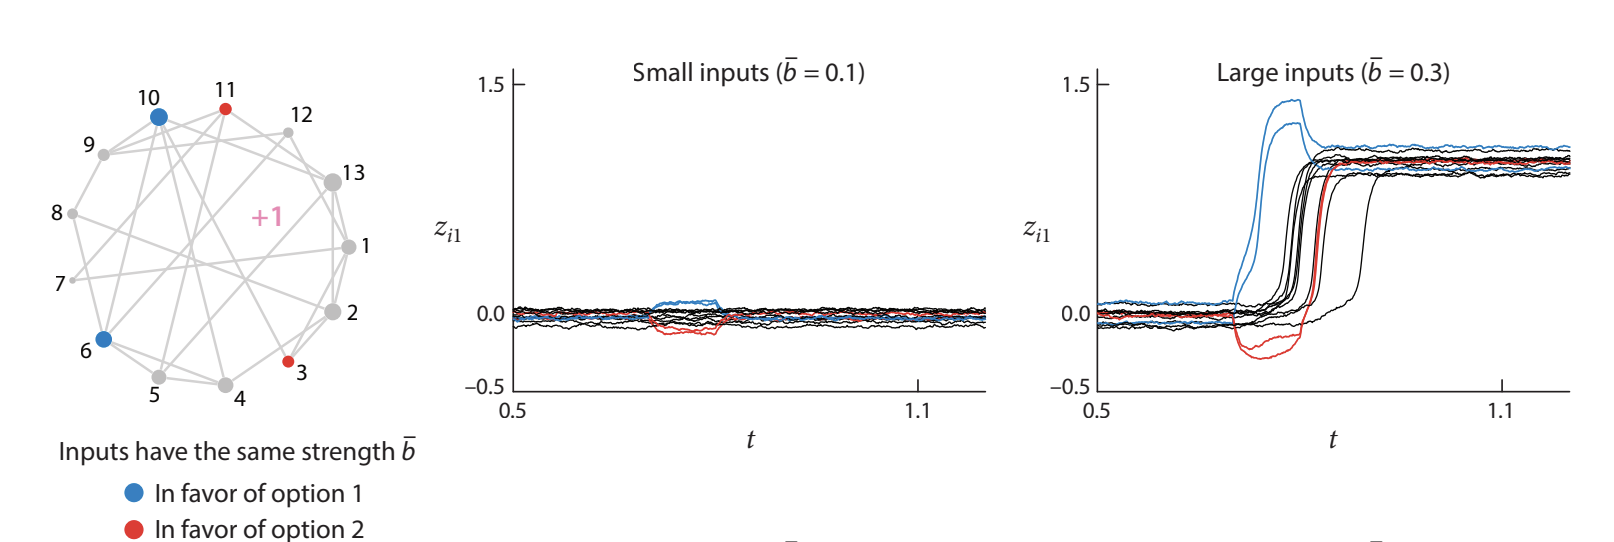
\includegraphics[width=\textwidth]{../plots/leonardfig2panA.png} 
		\caption{Results (Figure 2) of Leonard et al. 2024} \label{fig:damping1}
	\end{subfigure}
	
	\begin{subfigure}[t]{0.6\textwidth}
		\centering
		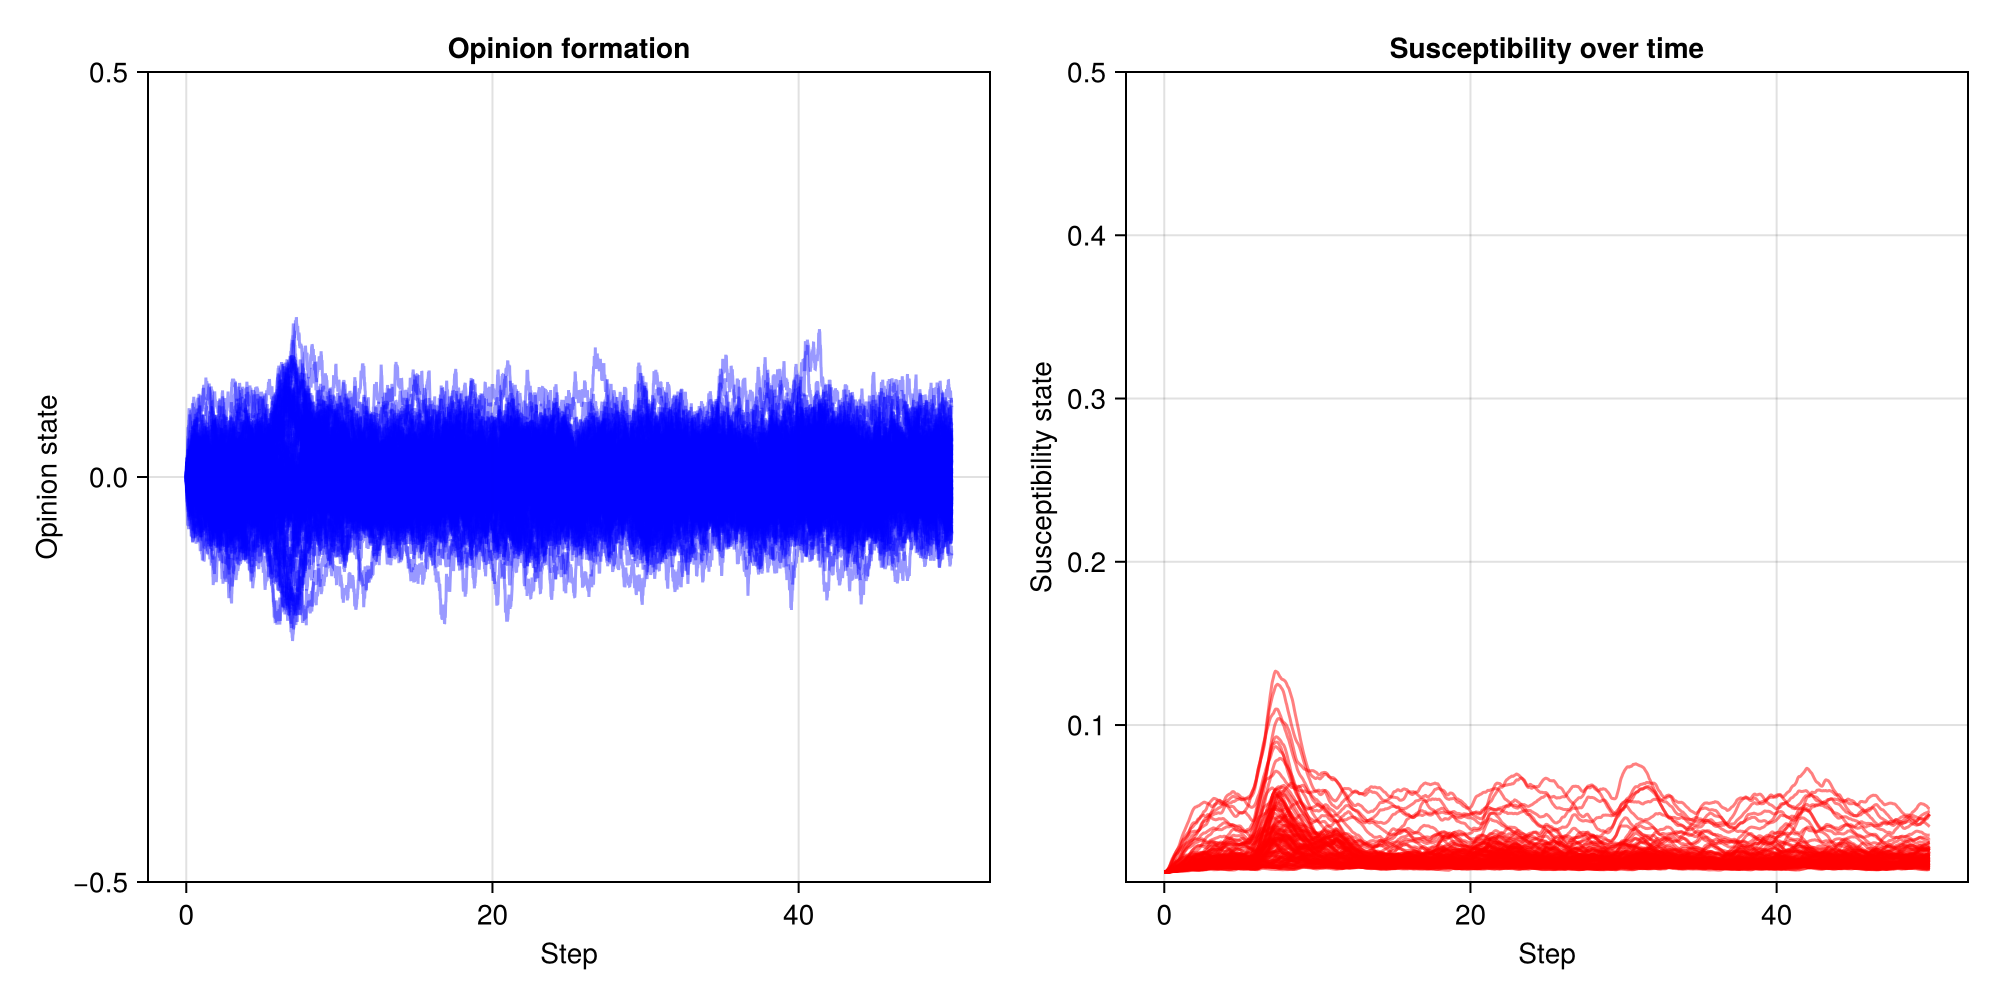
\includegraphics[width=\textwidth]{../plots/old/nog_constd_lowsig.png} 
		\caption{My simulation, input $b = \pm 0.1 $} \label{fig:damping2}
	\end{subfigure}
	
	\begin{subfigure}[t]{0.6\textwidth}
		\centering
		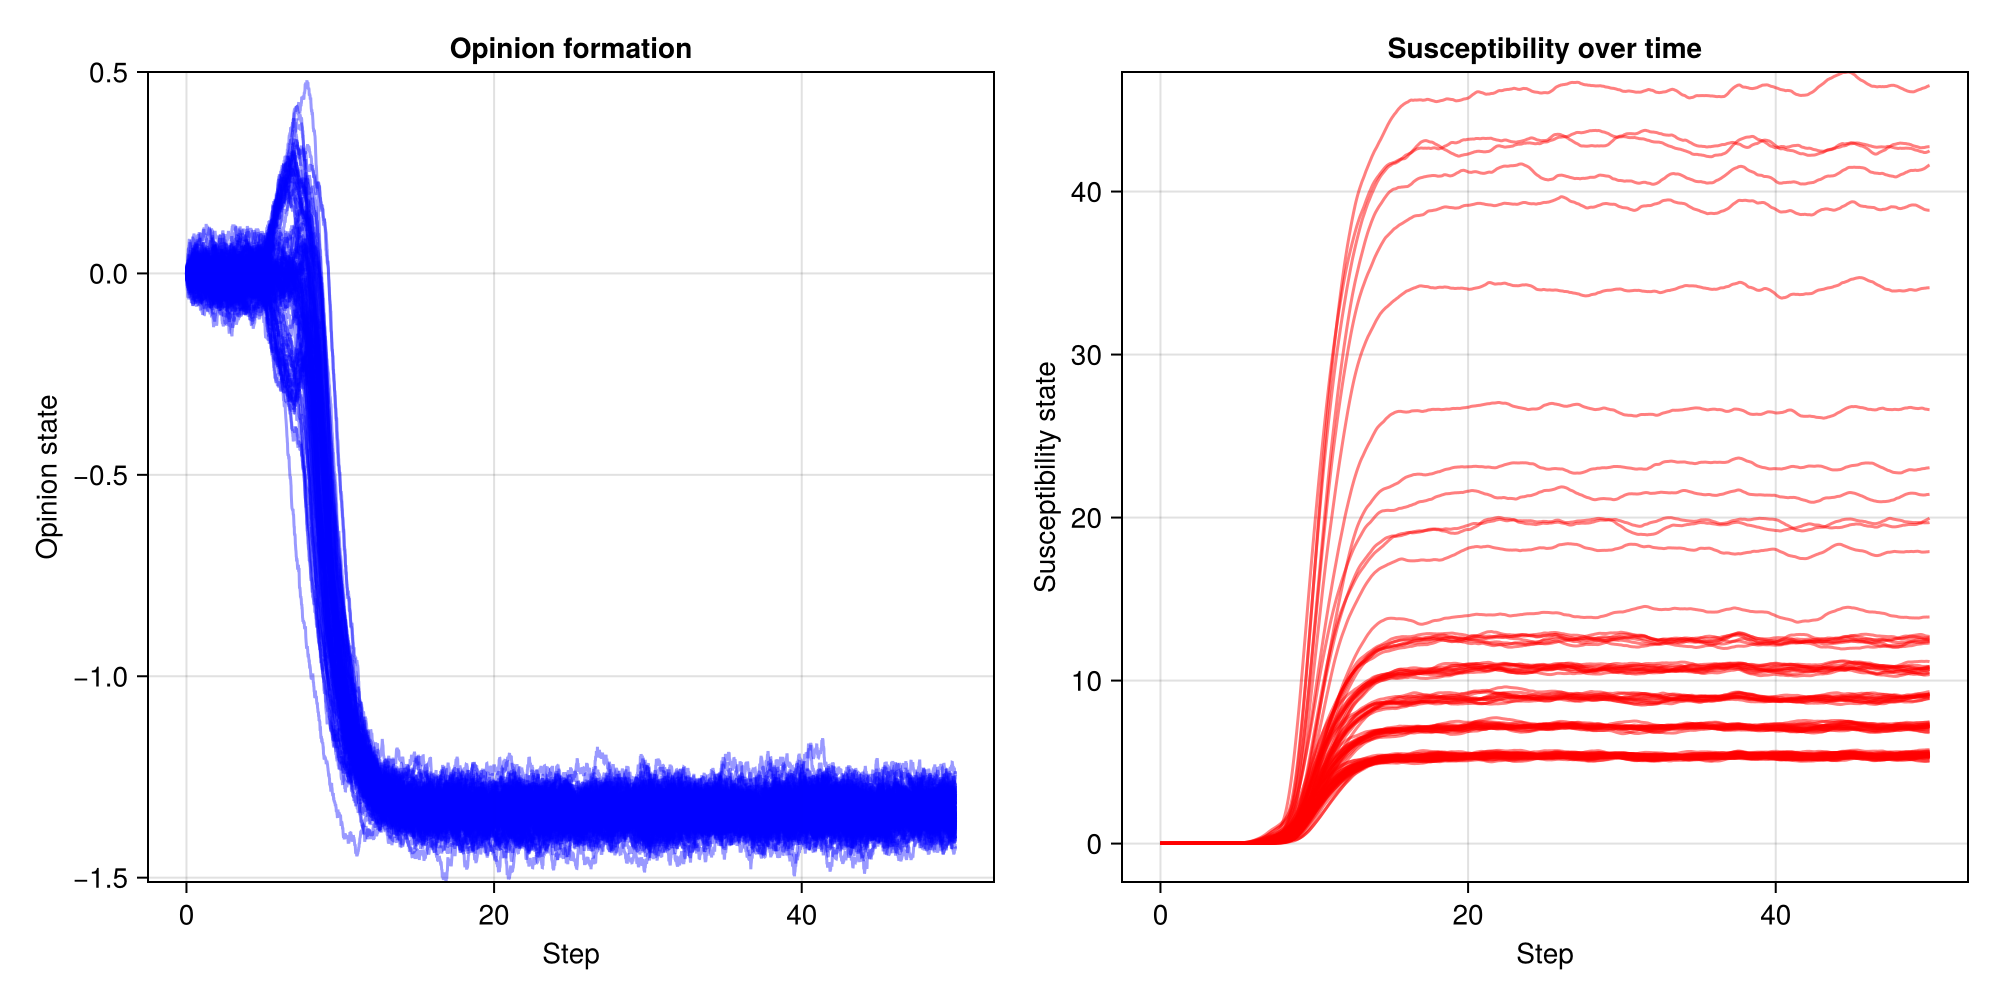
\includegraphics[width=\textwidth]{../plots/old/nog_constd_medsig.png} 
		\caption{My simulation, input $b = \pm 0.25 $} \label{fig:damping3}
	\end{subfigure}
	
	\caption{Opinion cascades under homogeneous damping and Gaussian noise, as external inputs grow larger. (\subref{fig:damping1}) is the top panel of Figure 2 of the BFL 2024 paper. In a small network of 13 agents, two agents receive a short signal of strength $b$ in favor of option 1 and concurrently, two agents receive a short signal of strength $-b$ in disfavor of option 1. Susceptibility state is not included. (\subref{fig:damping2}) and (\subref{fig:damping3}) are my simulations reproducing the same phenomena, with a network of 100 agents, with $d_i=d=0.75$. Opinion state in blue, susceptibility state in red. 25 agents receive a short signal in favor of option 1; 25 others receive a similar signal in disfavor. }\label{fig:replication}
\end{figure}

\textit{Sensitivity and robustness.} The authors also showed that at the bifurcation, indecision-breaking occurs rapidly, in a switch-like manner. As the system nears bifurcation, it becomes increasingly sensitive to certain inputs (in a selective manner). That is, it responds strongly to input vectors that align with the right eigenspace of the Jacobian at the bifurcation, but ignore input vectors that do not. Away from the bifurcation, opinion states remain stable even in the presence of small perturbations.

\textit{Stable disagreement.} The BFL model offered an elegant solution to a long-standing problem in the field of opinion formation: how to craft a system that may break indecision and generate stable disagreement as a function of inputs and initial conditions, rather than one that inevitably converges to consensus or avoids consensus only at the cost of a fixed, carefully hand-picked connectivity matrix (\cite{ravazziDynamicalSocialNetworks2021}, \cite{bernardoBoundedConfidenceOpinion2024}). This problem is sometimes called Abelson's diversity puzzle (\cite{abelsonMathematicalModelsDistribution1964}). 

\textbf{Assumptions of the BFL model.} A few things should be noted about the assumptions involved in this model.
\begin{enumerate}
	\item \textbf{Homogeneity.} Agents are homogeneous between each other (only their state distinguishes them) and across time (they do not learn or remember, only their state changes). For instance, agents all share a susceptibility time constant of $\tau^u$ and an opinion time constant of $1$. Agents all share an identical, non-parameterized input-output function. Agents all share a constant basal susceptibility and susceptibility gain. 
	\item \textbf{Balance of self-inhibition and recurrent excitation.} The self-inhibition implies that the opinion activation of each agent tends to revert to zero. This is balanced out by the self-excitation represented by the diagonal term of the $J^z$ matrix and the recurrent excitation represented by its non-diagonal terms, but modulated by the susceptibility state. At a low susceptibility, self-inhibition dominates and opinions tend to revert to zero. This is very close to the modeling of integrate-and-fire neurons.
	\item \textbf{Damping sets the opinion saturation levels.} While the damping coefficient $d_i$ is indexed as unit-specific, in most reported experiments, the original authors set a homogeneous value of $d_i=d$ for all agents. In the solution to the dynamical equations, $\pm d^{-1}$ becomes the scalar value of the stable opinionated states that the system may reach. That is, $d_i$ determines the value at which the opinion state of each agent $i$ will saturate. Diversity in $d_i$ would mean that instead of converging to identical scalar opinion states, agents would converge to opinion states of different magnitudes (agents are more or less convinced or extreme in their views). While this may seem realistic for social decision-making, this would be an artificial and hand-crafted way to achieve this result. Setting a homogeneous $d$ allows us to explore more interesting ways to achieve diversity.
	\item \textbf{Functional form and unboundedness of the susceptibility update.} It is not clear why the authors chose to square the opinion states in the susceptibility update. First, this assumes symmetry in the impact of negative and positive opinions, which is not obvious. I may not be equally affected by my friends being strongly in favor or in disfavor of something, although the difference between the two may be small enough that this does not impact results. In addition, because opinion states can grow larger than one (as determined by $d$ or the distribution of $d_i$) and the susceptibility update contains a sum of squared opinions, the susceptibility state can grow arbitrarily large.
\end{enumerate}

\subsection{Modified model}

\textbf{Adaptive time constants.} In real social networks, agents individually and dynamically adjust their reaction times, as they receive information from other agents and assess the state of the social system in which they are embedded. As a first step in modeling more complex agents, I add to the BFL model an adaptive time constant. In addition to better reflecting real social networks, the modified model should exhibit a richer dynamical range. Research on the physics of neural computation suggests that the nature of multiplicative interactions (or gating) in a model crucially determine its computational capabilities (\cite{krishnamurthyTheoryGatingRecurrent2022}). This change should allow the network to flexibly handle information on a range of time scales, and to enter regimes in which continuous attractors are formed. 

\textbf{Gated model.} I modify the model to include an input-dependent adaptive time-constant for the opinion update, in the form of a parameterized multiplicative gate that controls the rate of integration of the information received from the network (\cite{krishnamurthyTheoryGatingRecurrent2022}):

\begin{align}
	\dot{z}_{i}(t) &= \phi \left( x_i(t) \right) \cdot \left( -d_{i}z_{i}(t) + S \left( u_i(t) \cdot  \sum^{N}_{j=1} J^z_{ij}z_{j}(t)  \right) \right) + I_{i}(t) \\
	\tau^u \dot{u}_i(t) &=  -u_i(t)+u_0+g^u \sum ^{N}_{j=1} J^u_{ij}(z_{j}(t))^2 \\
	\tau^x \dot{x}_i(t) &= -x_i(t) +  \sum ^{N}_{j=1} J^x_{ij} S(z_j(t)) + k_i I_i(t)
\end{align}

\textbf{Definitions.} $J^x$ is a coupling matrix for the gate, $\phi (x) = (1 + e^{- \alpha x + \beta })^{-1}$ is a sigmoidal saturation paramaterized by $\alpha$ and $\beta$, and $k_i I_i$ is a scaled version of $I_i$.

\subsection{Simulations}

In my simulations, I examined how gating impacts indecision-breaking bifurcations after the reception of contradictory signals of similar strengths. In all cases, one fourth of the agents receive a burst of positive signal, and another fourth concurrently receive a burst of negative signal. I compared the initial and gated models while varying the \textbf{strength of inputs} (low, medium, or high signal) and the \textbf{type of connectivity matrix} (random, scale-free, or small-world; see below).

For now, I simulated the system's evolution using the Julia Agent.jl package and Euler's approximation with a step size $h = 0.01$. I plan to replicate the results later using differential equations solvers and higher order approximations methods.

All results are preliminary, as I have only had time to reproduce them with a couple of different seeds, and robustness across a variety of random seeds should be verified.

\textbf{Parameters for the simulations.} Some parameters must be held constant to focus on the effect of gating, signal strength, and connectivity. I set $N = 100$, which should be sufficient to generate graphs that are structurally distinct while remaining computationally tractable. After some exploration of the model's behavior in various regimes, I set the parameters as follows for all simulations in this report. $\tau^u = 1$, $g^u = 0.5$, $u_0=0$, $\tau^x = 5$, $\alpha = 2$, and $\beta = 0$. The damping coefficient is set constant at $d_i = d = 0.75$ and the scaling factor is sampled from a Gaussian, $k_i \sim \mathcal{N}(1,0.25)$, to create heterogeneity across agents. Any of these assumptions may be relaxed or modified in future work. 

\textbf{Connectivity matrices $J^a$, $J^u$ and $J^x$.} For now, I set $J^a = J^u = J^x$, with the assumption that agents are both communicating with and paying attention to the same other agents (e.g. their friends). I also assume that $J^a$ is symmetric, which corresponds to the social graph being undirected.

It might be particularly interesting to vary both assumptions in future work. The first, for instance, to allow agents to have through the gating matrix some perception of the state of the broader social system in which they are embedded, and adjust their integration time accordingly. The second, to allow for unidirectional flow of information between agents.

I examine the dynamics associated with three different types of social graphs: Erdős-Rényi $G(n, M)$ (ER), Barabási-Albert (BA), and Watts-Strogatz (WS). I set the parameters of each of the three generators such that the average degree is comparable.\footnote{$N = 100$ agents. For ER, $M = N*3$ and $N*4$. For BA, $k = 3$ and $4$. For WS, $k = 6$ and $8$, $\beta = 0.1$.} ER is a classic random graph model without hubs or local clusters. BA is a scale-free network based on preferential attachment and has a power law degree distribution (and hence hubs). WS has a small-world structure and hence local clusters. While none is a perfectly realistic depiction of social networks, together they cover an interesting range of network structures.

\begin{figure}
	\begin{subfigure}{0.45\textwidth}
		\centering
		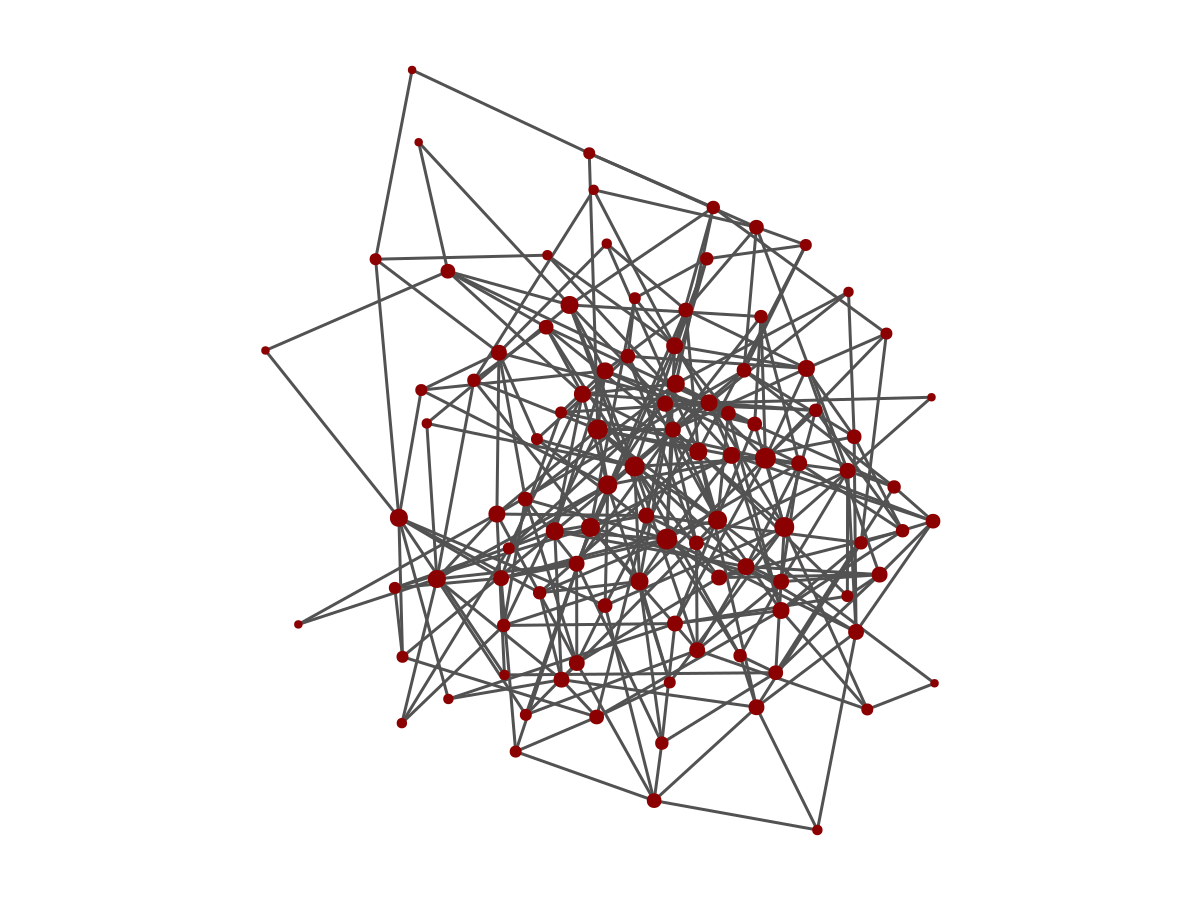
\includegraphics[width=0.9\linewidth]{../plots/g_erdosrenyi_n100_p3_s33} 
		\caption{ER graph}  \label{fig:subim11}
	\end{subfigure}
	\hfill
	\begin{subfigure}{0.45\textwidth}
		\centering
		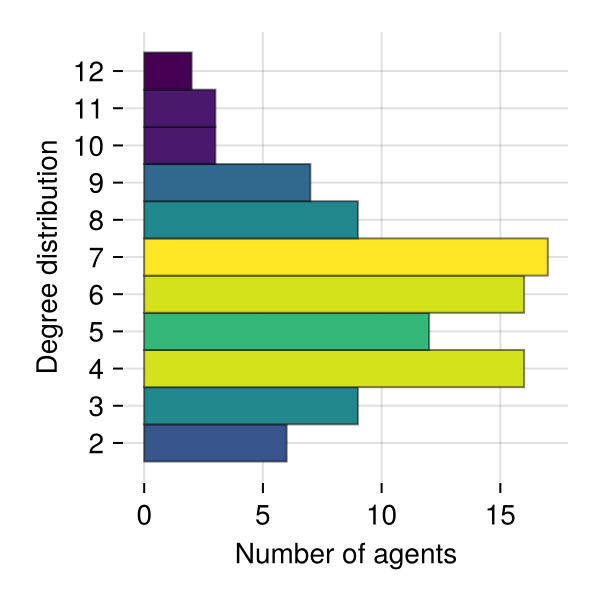
\includegraphics[width=0.7\linewidth]{../plots/g_erdosrenyi_hist_degree_n100_p3_s33}
		\caption{ER degree distribution} \label{fig:subim12}
	\end{subfigure}
	
		\begin{subfigure}{0.45\textwidth}
		\centering
		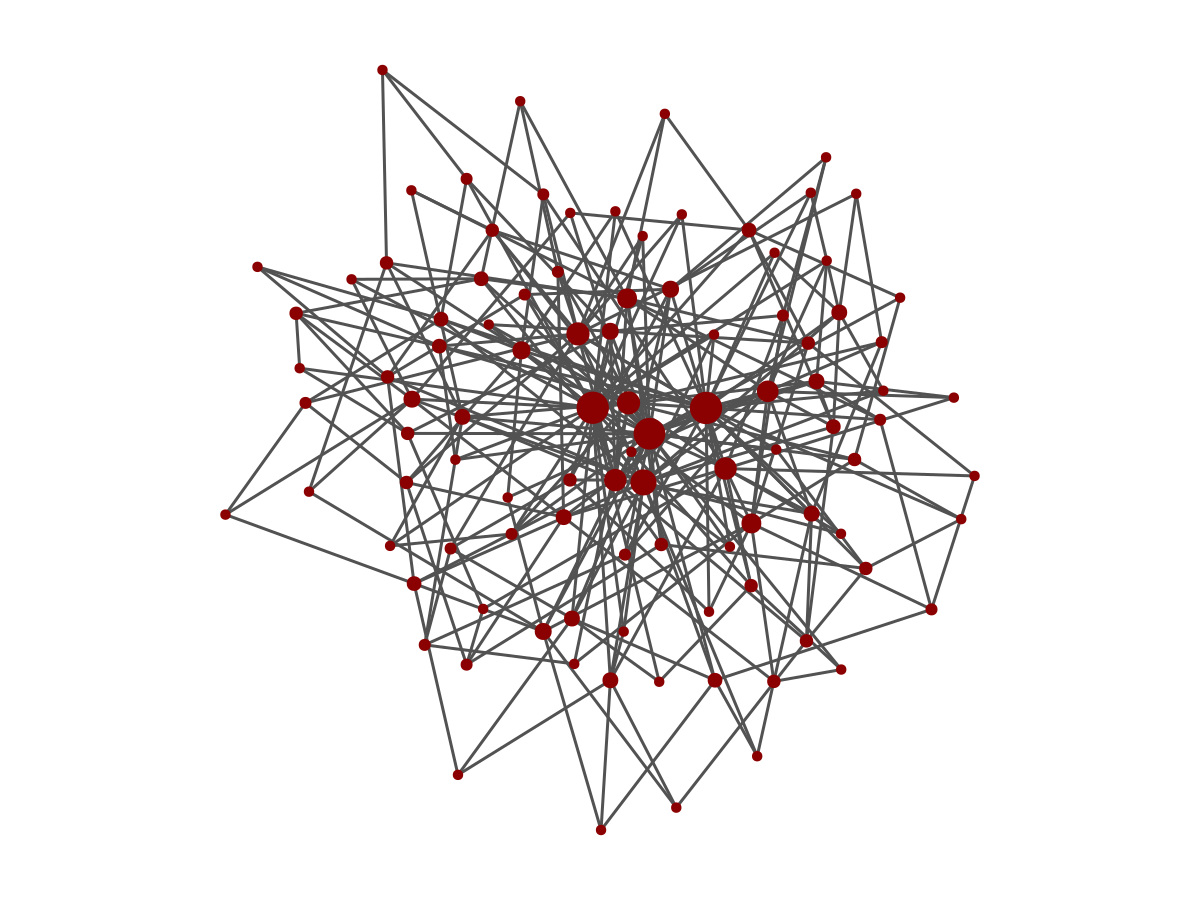
\includegraphics[width=0.9\linewidth]{../plots/g_barabasialbert_n100_m3_s33} 
		\caption{BA graph}  \label{fig:subim21}
	\end{subfigure}
	\hfill
	\begin{subfigure}{0.45\textwidth}
		\centering
		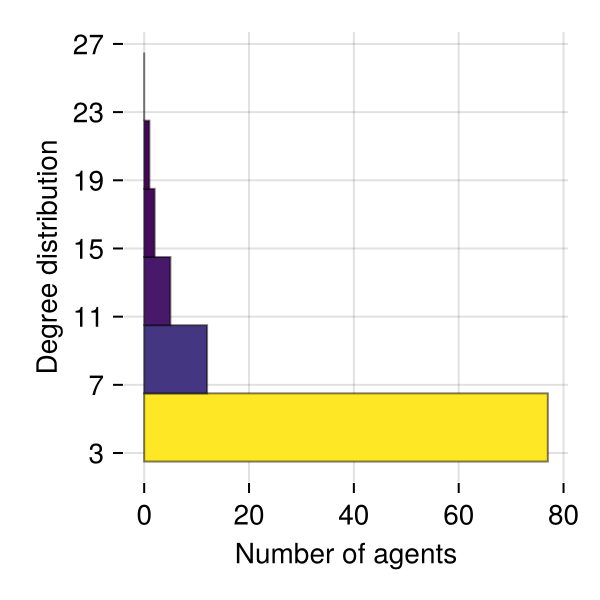
\includegraphics[width=0.7\linewidth]{../plots/g_barabasialbert_hist_degree_n100_m3_s33}
		\caption{BA degree distribution} \label{fig:subim22}
	\end{subfigure}
	
		\begin{subfigure}{0.45\textwidth}
		\centering
		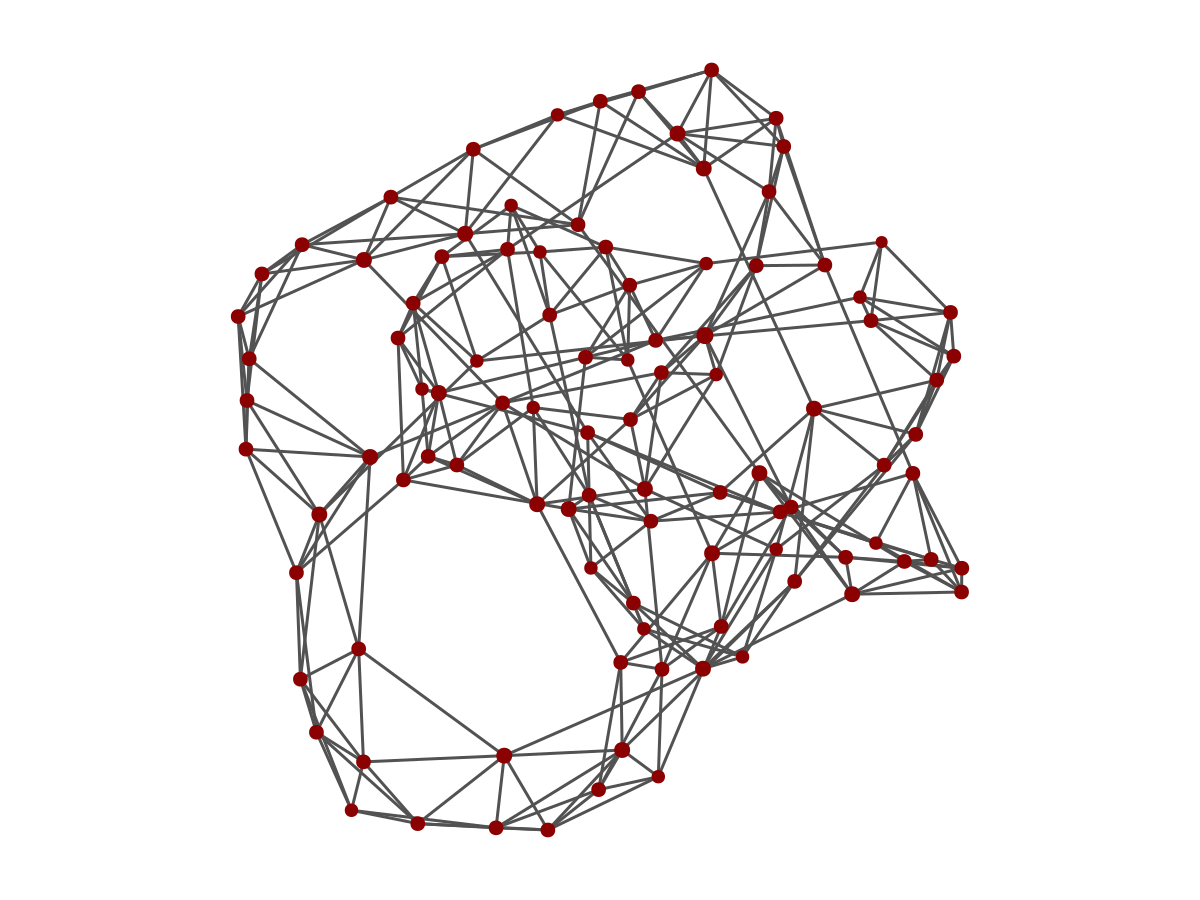
\includegraphics[width=0.9\linewidth]{../plots/g_wattsstrogatz_n100_k3_p01_s33} 
		\caption{WS graph}  \label{fig:subim31}
	\end{subfigure}
	\hfill
	\begin{subfigure}{0.45\textwidth}
		\centering
		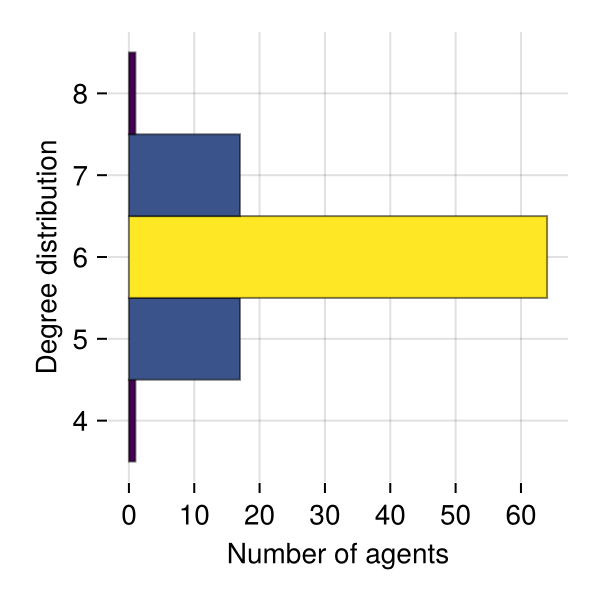
\includegraphics[width=0.7\linewidth]{../plots/g_wattsstrogatz_hist_degree_n100_k3_p01_s33}
		\caption{WS degree distribution} \label{fig:subim32}
	\end{subfigure}
	
	\caption{Example structure for the three types of social graphs explored in simulations.}
	\label{fig:graphtypes}
\end{figure}

Figure \ref{fig:graphtypes} illustrates this range by depicting a randomly generated graph of each type, along with its degree distribution.



\subsubsection{Initial conditions}
Agents are initialized at the basal susceptibility, $u_i = 0.01$, and at a random, almost neutral opinion state $z_i \sim \mathcal{N}(0, 0.01)$.

Gating states are initialized at zero.



\section{Results and discussion}






\newpage

\section{Future directions}

\textbf{Further modifications to the model.}


\textbf{Building predictive models of the environment from partial information.} Building predictive models of their environment is a crucial component collective intelligence. Here, I take model building to mean the discovery of structure and regularity in a dynamic environment so that a system can predict its next inputs better than at random; such models can be implicit and behavioral (\cite{crutchfieldCalculiEmergenceComputation1994}). In real social networks, the information acquired by agents in order to do so is not only noisy, it is also partial and heterogeneous across agents. Settings of partial and heterogeneous information have rarely been explicitly studied in the network dynamics literature.

Ongoing research efforts (\cite{malachAutoRegressiveNextTokenPredictors2023}) suggest that in some settings, next-token prediction of structured sequences may enable a model to learn complex data-generating processes (DGP) accurately. However, if and how a DGP can be recovered by a network when different nodes each receive noisy and imperfect measurements of the sequences remains unknown.

The BFL model only examines subjective beliefs, not the ability to converge to correct or useful answers. In the future, I plan to change the task from belief propagation to the collective recovery of a model of the environment from partial and heterogeneous information. A ground truth will exist, and I will examine under what conditions the network is successful at recovering it from noisy, partial and asymmetric inputs, including varying the distribution of information, noise, and other system parameters. This will be formalized in two ways, first as a static matrix reconstruction problem, and then as a dynamic hidden Markov problem.

Interacting adaptive agents face some collective challenges that resemble those of neurons in the brain or nodes in an artificial network: (i) implementing distributed computation robustly and flexibly, over a range of time scales, and (ii) building predictive models of their environment. Together, I call tackling those goals collective intelligence. If there exists common principles underlying collective intelligence across settings, then models of neural computation may help us understand social computation. Conversely, models of social computation between complex agents might in turn suggest new models for how groups of neurons or regions of the brain interact to create a richer dynamical repertoire.

\printbibliography[heading=bibintoc, title={References}]

\newpage

\appendix

\section{Simulation results}



\end{document}